%%
%% Capítulo 2: Expressões matemáticas
%%

\mychapter{Desenvolvimento da solução}
\label{Cap:desenvolvimento-da-solucao}

A principal característica do Windbox é a disponibilização de análises, realizadas sobre os dados dos aerogeradores fornecido no sistema SCADA, para que os gestores dos parques eólicos possam identificar rapidamente desvios na produção e corrigi-los em tempo hábil. Para a criação destas análises, o Windbox utiliza como base as normas técnicas internacionais de energia eólica desenvolvidas pelo Comitê Técnico 88 da Comissão Eletrotécnica Internacional (International Electrotechnical Commission - IEC). 

Nesta seção será discutido as principais características técnicas que estão presentes no Windbox: normas da IEC, tecnologias utilizadas e o modelo de negócio.

\section{Nomas da IEC}
\label{Sec:normas-iec}

Em 1987 o Comitê Internacional de Eletrotécnica (IEC) criou a comissão técnica 88 (TC 88) com a ideia de padronizar assuntos relacionados a turbinas eólicas. A norma originada foi a IEC 61400 e especifica os requisitos essenciais de projeto, fabricação, instalação operação e manutenção. O seu principal objetivo é disponibilizar um nível adequado de proteção contra danos causados por todo tipo de risco durante a vida útil prevista dos equipamentos. Ela abrange todos os subsistemas de um turbina eólica e se aplica a todos os tamanhos de aerogeradores.

A norma da IEC 61400 está dividida em várias partes, cada uma delas com um determinado título e assunto. As que estão atualmente em vigor são:

\begin{itemize}
    \item IEC 61400-1: Requisitos de projeto (\textit{Design requirements})
    \item IEC 61400-2: Pequenas turbinas eólicas (\textit{Smallwind turbines})
    \item IEC 61400-3: Requisitos de projeto para turbinas eólicas offshore (\textit{Design requirements for offshore wind turbines})
    \item IEC 61400-4: Requisitos de projeto para caixas de engrenagens de turbinas eólicas (\textit{Design requirements for wind turbine gearboxes})
    \item IEC 61400-5: Pás do rotor da turbina eólica (\textit{Wind turbine rotor blades})
    \item IEC 61400-11: Técnicas de medição de ruído (\textit{Acoustic noise measurement techniques})
    \item IEC 61400-12: Medições do desempenho de potência de aerogeradores (\textit{Wind turbine power performance testing})
    \item IEC 61400-13: Medição de cargas mecânicas (\textit{Measurement of mechanical
loads})
    \item IEC 61400-14: Indicação de níveis aparentes de potência sonora (\textit{Declaration of apparent sound power level and tonality values})
    \item IEC 61400-21: Medição e avaliação das características da qualidade da energia de aerogeradores conectados à rede (\textit{Measurement and assessment of power quality characteristics of grid connected wind turbines})
    \item IEC 61400-22: Teste de conformidade e certificação (\textit{Conformity testing and certification})
    \item IEC 61400-23: Teste estruturais em larga escala das pás do rotor (\textit{Full-scale structural testing of rotor blades})
    \item IEC 61400-24: Proteção contra descargas atmosféricas (\textit{Lightning protection})
    \item IEC 61400-25: Protocolo de comunicação (\textit{Communication protocol})
    \item IEC 61400-26: Disponibilidade de tempo com base em turbinas eólicas (\textit{Time basedavailability for wind turbines})
    \item IEC 61400-27: Modelos de simulação elétrica para o gerador eólico (\textit{Electrical simulation models for Wind power generation})
\end{itemize}

O Windbox faz uso da IEC 61400-12 e da IEC 61400-26. A primeira, define as técnicas para medição da potência de geração. Já a segunda, define termos genéricos para descrever a disponibilidade do aerogerador e seus componentes, além da expectativa de vida e critérios para determinar os intervalos de manutenção das turbinas.   

O principal objetivo da IEC 61400-12 é a definição da curva de potência do aerogerador. A curva de potência apresenta a relação entre a velocidade do vento incidente sobre o rotor e a potência elétrica gerada pelo aerogerador, como comentado na seção \ref{Sec:desempenhoDeAerogeradores}. Com esse dado é possível extrair indicadores de desempenho e saber se o aerogerador está gerando energia, para as condições de vento encontradas, conforme foi especificado pelo fabricante.

Como foi dito na seção \ref{Sec:disponibilidadeDesempenhoAerogeradores}, a disponibilidade de um aerogerador pode ser interpretada de diferentes formas na visão dos fabricantes (disponibilidade técnica) e dos proprietários de parques (disponibilidade operacional). A principal diferença entre esses dois conceitos está na classificação de cada parada do aerogerador. A IEC 61400-26 veio para padronizar e catalogar os estados que um aerogerador pode assumir  durante a sua operação, para que possa ser atingido um nível de consenso aceitável nas discussões sobre disponibilidade entre os fabricantes e os proprietários de parques.

\section{Tecnologias utilizadas}
\label{Sec:tecnologias}

%% Falar que é uma solução em nuvem.

O Windbox é uma solução que realiza análise sobre os dados dos aerogeradores fornecido no sistema SCADA. Todo o sistema é baseado em computação em nuvem, ou seja, o cliente do Windbox não necessita de uma infraestrutura própria para adquirir a solução. Uma das etapas mais importantes do sistemas consiste ma na coleta dos dados. Segundo \citeasnoun{integracao-sistemas-scada}, no meio industrial, o sistema SCADA pode disponibilizar diversos tipos de protocolos de comunicação para acesso aos dados, como por exemplo: ODBC, DNP3, OPC e Modbus. 

No Windbox, a coleta dos dados do SCADA é realiza através do módulo \textit{Windbox Collector}. Nesse módulo estão implementados alguns dos mais comuns protocolos de comunicação, como por exemplo: OPC Classic, OPC UA, ODBC e IMAP. No setor de energia eólica o principal protocolo utilizado pelo Windbox é o OPC.

O OPC é um protocolo de conectividade de dados baseado nos populares padrões COM/DCOM de comunicação da \textit{Microsoft}. O OPC Classic, nome dado ao primeiro padrão criado, foi idealizado com a proposta de facilitar a conectividade entre os diversos dispositivos de chão de fábrica (SCDs, CLPs, etc) e as aplicações de software (SCADA, historiadores, etc), padronizando a forma de comunicação entre eles. Há diversas especificações de OPC Classic adequadas às diferentes situações de uso de dados: OPC DA (Data Access) para dados instantâneos, OPC HDA (Historical Data Access) para dados históricos e OPC A\&E (Alarms and Events) para dados de alarmes e eventos. Nos dias atuais o OPC Classic vem dando espaço ao OPC UA, versão mais atual do OPC que vem se tornando cada vez mais popular nas industrias devido a facilidade de uso e a compatibilidade com outros sistemas operacionais.

Com a informação do sistema SCADA sendo coletada pelo \textit{Windbox Collector}, os dados precisam ser armazenados. Nesse caso o módulo responsável no sistema por essa função é o \textit{Windbox Data Base}. Neste módulo encontra-se uma das maiores inovações do Winbdox.

Tomando como exemplo um único parque eólico com 15 aerogeradores, este parque enviaria diariamente para o windbox cerca de 65 mil registros. Em um ano de operação seriam cerca de 23 milhões 725 mil registro. O cenário piora quando se pensa em 10 ou 100 parques. É uma quantidade de dados muito grande e que precisa de uma solução robusta para atender a essa demanda. Pensando nisso, foi desenvolvido uma estrutura de armazenamento de dados similar ao Athenas Historian, utilizando como base o banco de dados Apache Cassandra. O Cassandra é um O banco de dados NoSql, orientado a coluna que foi originalmente desenvolvido pelo Facebook e hoje é mantido pelo Apache como uma plataforma \textit{open source}. É uma solução que foi projetada para funcionar em hardwares de baixo custo e tem como principal objetivo lidar com a alta taxa de requisições de gravação sem perder a eficiência da leitura \cite{cassandra-banco-dados}.

Uma das principais características do módulo de armazenamento é que ele pode ser constituído por diversos serviços de armazenamento de forma descentralizada, em cluster, permitindo com isso dividir a carga de processamento e armazenamento dos dados entre os nós do sistema. Esta característica distribuída permite que o sistema consiga escalar de acordo com a necessidade. A figura \ref{Fig:moduloArmazenamentoDados} ilustra a arquitetura descentralizada do Windbox.

\begin{figure}[htbp!] \begin{center}
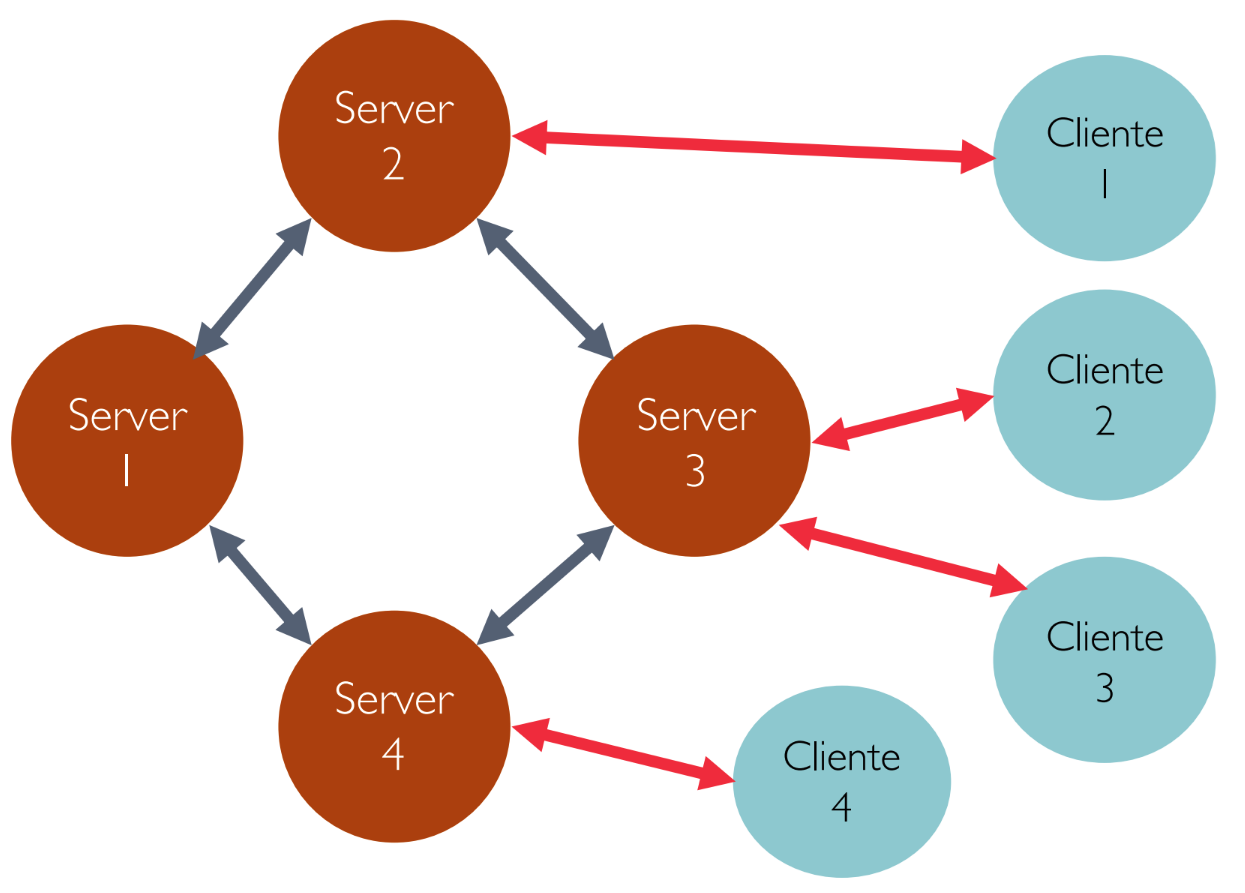
\includegraphics[width=0.75\linewidth]{./figuras/arquitetura-banco-de-dados-windbox}
\caption{Arquitetura do módulo de armazenamento de dados do Windbox}
\label{Fig:moduloArmazenamentoDados}
\end{center} 
\end{figure}

Após os dados serem armazenados no \textit{Windbox Data Base}, eles precisar ser tratados e analisados para disponibilizar os indicadores aos usuários. Essa é a função do módulo \textit{Windbox Analyse}. Desenvolvido na linguagem de programação SCALA, esse módulo tem como principal característica o rápido processamento dos dados fornecidos pelo módulo de armazenamento. Scala é uma linguagem de programação para aplicações de software em geral, que combina os paradigmas de programação orientada a objetos e funcional e que tem como uma das principais características, a facilidade de trabalhar com programação concorrente. Algumas dos indicadores fornecidas por esse módulo são: 

\begin{itemize}
    \item Indicador de produção potencial: Indica o quanto um complexo, parque ou aerogerador deveria ter produzido de energia em um dado período.
    \item Indicador de produção real: Indica o quanto um complexo, parque ou aerogerador produziu de energia em um dado período.
    \item Indicador de perda de produção: Indica o quanto um complexo, parque ou aerogerador perdeu de energia em um dado período.
    \item Indicador de disponibilidade: Indica a disponibilidade de um complexo, parque ou aerogerador em um dado período.
    \item Indicador de disponibilidade: Indica o quanto um complexo, parque ou aerogerador deveria ter produzido de energia em um dado período.
\end{itemize}

Esses são os principais indicadores fornecidos pelo Windbox. Com esses indicadores, os gestores dos parques podem visualizar as perdas que estão tendo em cada complexo, parque ou aerogerador. Identificando as perdas, o próximo passo é identificar a causa raiz responsável por isso. Para isso o Windbox fornece uma série de forma visuais de análise dos dados brutos do aerogerador, Uma dela é a visualização da curva de potência do aerogerador. Segundo \citeasnoun{tecnica-analise-dados-parque-eolico}, a análise de curva de potência é o método mais utilizado para medir o desempenho de um aerogerador. Como descrito na seção \ref{Sec:curvaDePotencia}, a curva de potência é representada pela velocidade do vento x a potência do aerogerador. Comparando a curva gerada por essas duas variáveis com a curva de referência do aerogerador, é possível verificar o comportamento do aerogerador de uma maneira geral, logo, um aerogerador que possui uma curva de potência parecida com a curva de potência garantida pelo fabricante deve estar me bom estado de funcionamento. Na figura \ref{Fig:curvaPotenciaNormal} pode ser visualizado uma curva de potência para um aerogerador com funcionamento considerado normal e na \ref{Fig:curvaPotenciaProblema} uma curva de potência para um aerogerador com funcionamento considerado anormal.

\begin{figure}[htbp!] \begin{center}
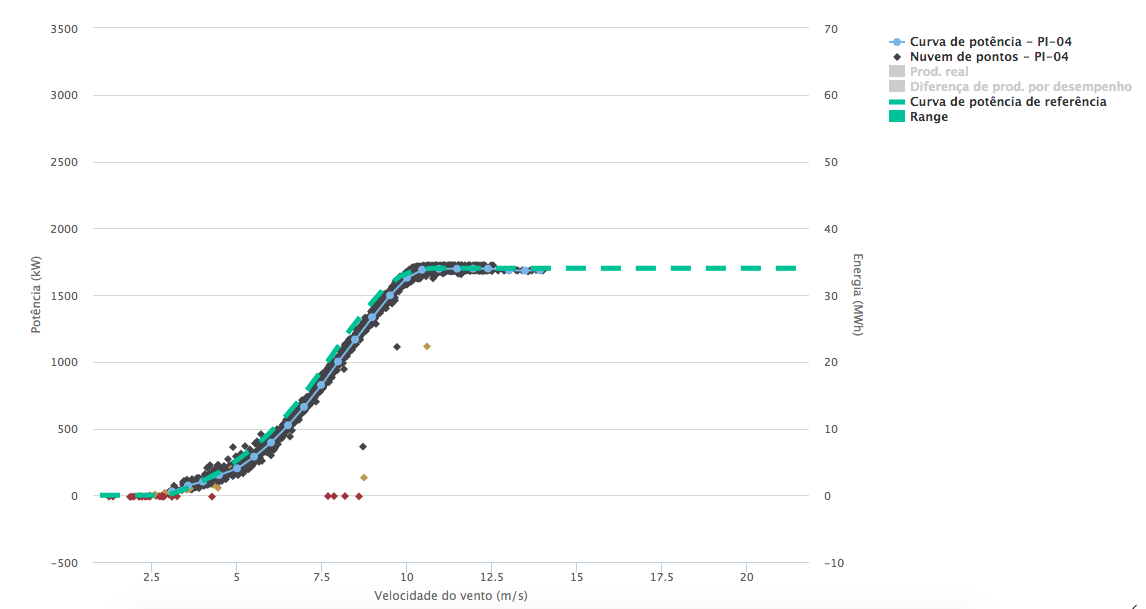
\includegraphics[width=1\linewidth]{./figuras/curva-potencia-normal}
\caption{Curva de potência considerada normal}
\label{Fig:curvaPotenciaNormal}
\end{center} 
\end{figure}

\begin{figure}[htbp!] \begin{center}
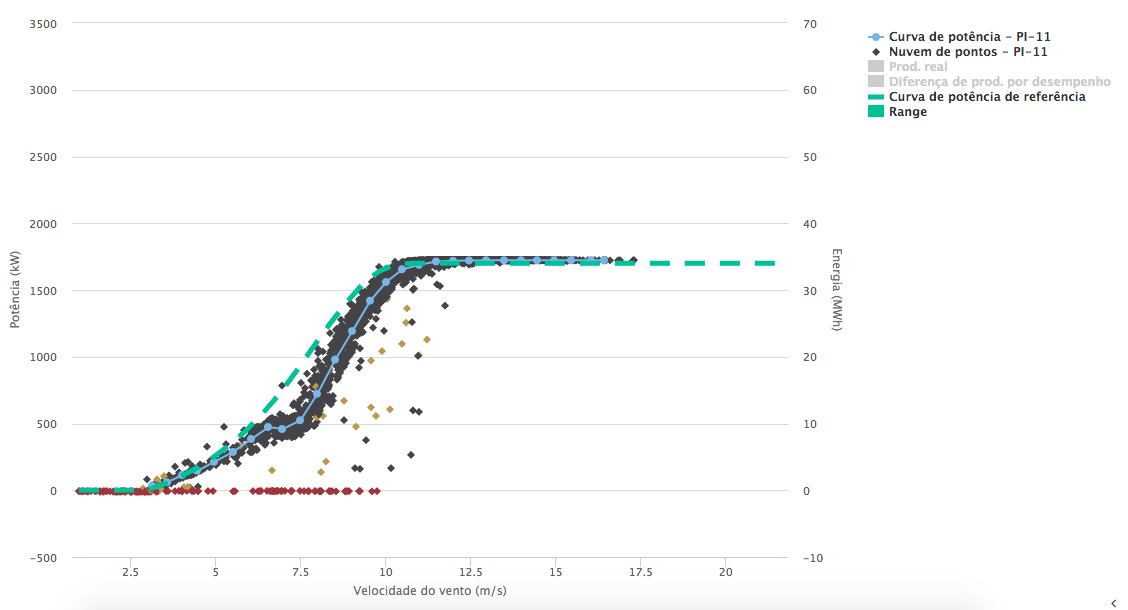
\includegraphics[width=1\linewidth]{./figuras/curva-potencia-problema}
\caption{Curva de potência considerada anormal}
\label{Fig:curvaPotenciaProblema}
\end{center} 
\end{figure}

Para que seja possível visualizar os dados disponibilizados pelo módulo \textit{Windbox Analyse}, o usuário conta com o módulo web. Esse módulo é responsável por organizar em \textit{dashboards} os gráficos com os indicadores e fornece ao usuário 3 níveis para visualização: complexo, parque e aerogerador. Isso possibilita que o gestor possa navegar entre uma análise macro da produção até uma micro. Nas figuras \ref{Fig:visualizaçãoNivelComplexoEolico}, \ref{Fig:visualizaçãoNivelParqueEolico}, \ref{Fig:visualizaçãoNivelAerogerador}, são demonstrados alguns indicadores nos três níveis de visualização.

\begin{figure}[htbp!] \begin{center}
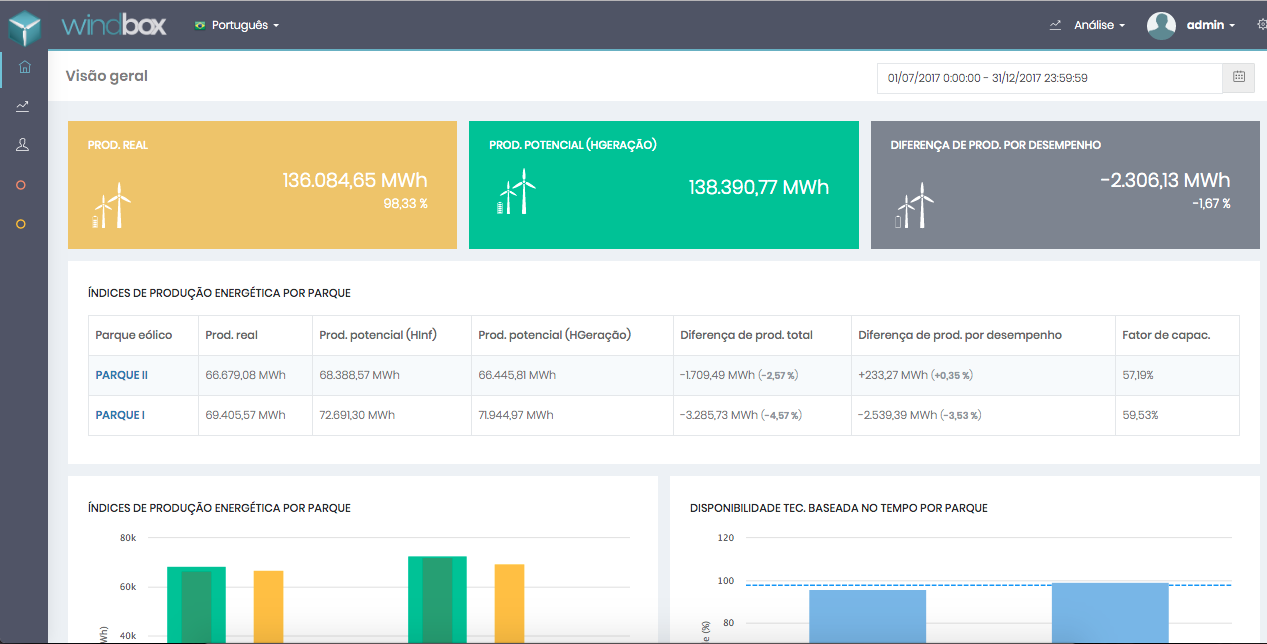
\includegraphics[width=1\linewidth]{./figuras/tela-complexo}
\caption{Visualização do Windbox a nível de complexo eólico}
\label{Fig:visualizaçãoNivelComplexoEolico}
\end{center} 
\end{figure}

\begin{figure}[htbp!] \begin{center}
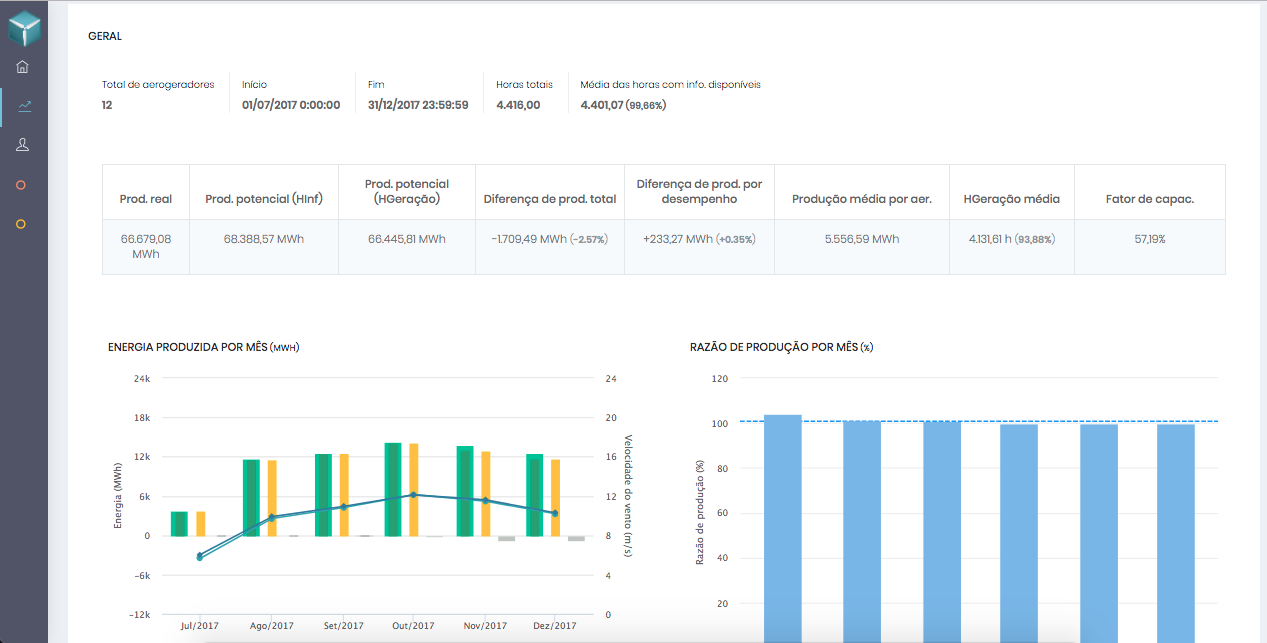
\includegraphics[width=1\linewidth]{./figuras/tela-parque}
\caption{Visualização do Windbox a nível de parque eólico}
\label{Fig:visualizaçãoNivelParqueEolico}
\end{center} 
\end{figure}

\begin{figure}[htbp!] \begin{center}
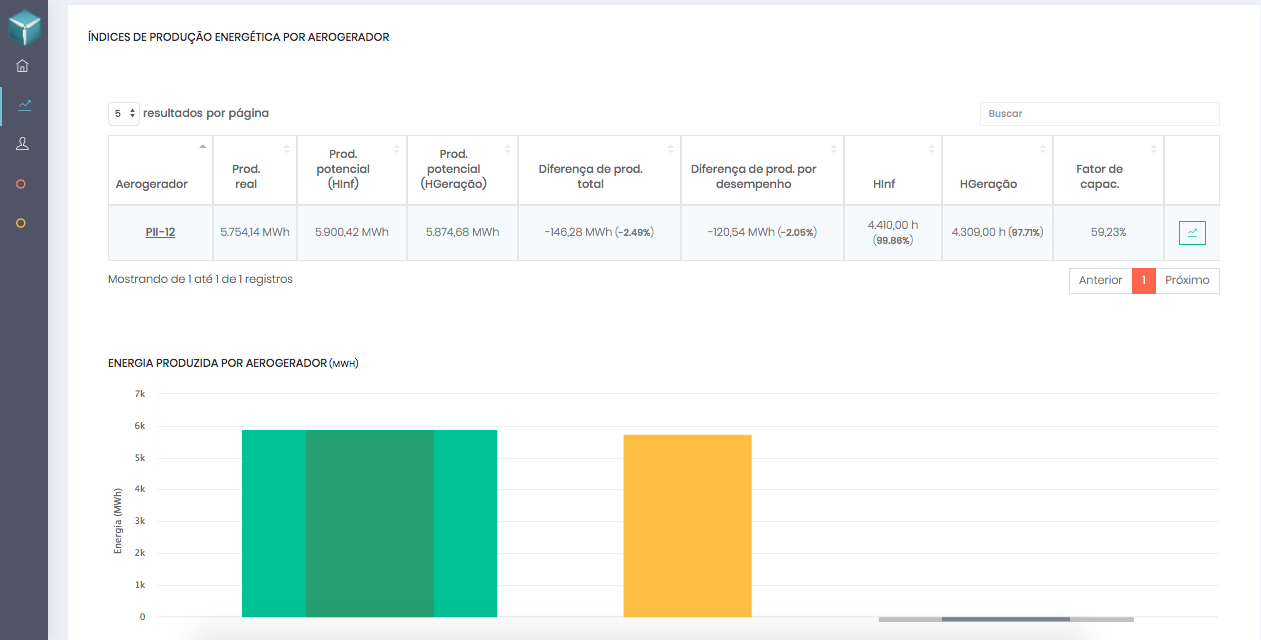
\includegraphics[width=1\linewidth]{./figuras/tela-aerogerador}
\caption{Visualização do Windbox a nível de aerogerador}
\label{Fig:visualizaçãoNivelAerogerador}
\end{center} 
\end{figure}

Na figura \ref{Fig:arquiteturaWindbox}, é demonstrado a arquitetura em camadas do Windbox. O protocolo de comunicação entre uma camada e outra muda de acordo com a necessidade. 

\begin{figure}[htbp!] \begin{center}
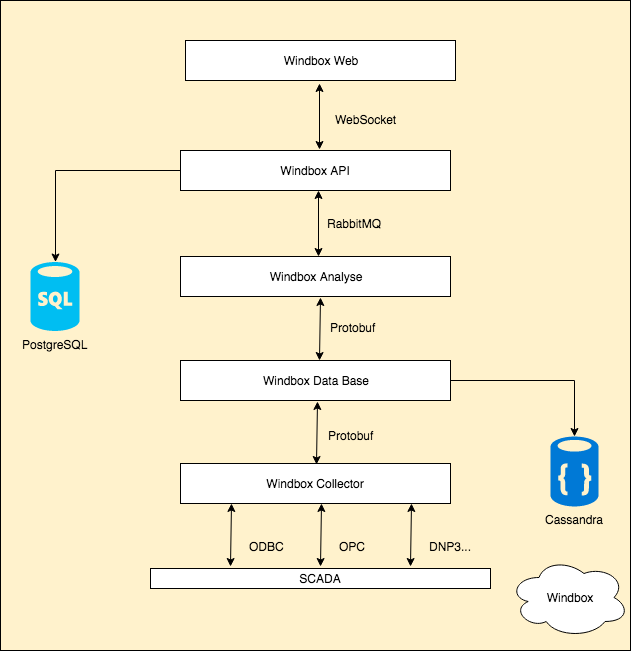
\includegraphics[width=0.75\linewidth]{./figuras/arquitetura-windbox}
\caption{Arquitetura em camadas do Windbox}
\label{Fig:arquiteturaWindbox}
\end{center} 
\end{figure}

Após a coleta pelo \textit{Windbox Collector}, o dado é enviado para o módulo \textit{Windbox Data Base} através do protocolo de comunicação \textit{Protobuf}. O \textit{Protobuf} é um protocolo criado pelo Google para serializar dados estruturados, independente de plataforma \cite{protobuf-google}. O grande motivo do Windbox estar utilizando esse protocolo para comunicação é que, segundo \citeasnoun{protobuf-dzone}, ele pode ser até 10 vezes mais rápido que o JSON. Como a quantidade de dados trafegado por esse módulo é alta, justifica essa necessidade. Após o envio do dado para o \textit{Windbox Data Base}, este dado fica disponível para o \textit{Windbox Analyse} realizar consultas. Mas uma vez se fez necessário o uso do \textit{Protobuf}, já que a quantidade de dados enviados para o módulo de análise é muito grande e necessita-se de um protocolo com ótimo desempenho.

Para que os dados brutos dos aerogeradores são analisados cada vez que um usuário requisita tal ação por meio de um componente gráfico no \textit{Windbox Web}. Essa requisição é enviada para o \textit{Windbox API} por meio de um \textit{WebSocket}. \textit{WebSocket} é uma tecnologia que torna possível abrir uma sessão de comunicação interativa ente o navegador do usuário e um servidor (no caso o \textit{Windbox API}). Com isso o \textit{Windbox Web} envia mensagens para o \textit{Windbox API} e recebe a resposta orientada ao evento de fim de processamento da análise de forma assíncrona. Dessa forma, cada componente gráfico de análise é carregado de forma independente. 

Com a requisição de análise feita para no \textit{Windbox API}. Este por sua vez tem a responsabilidade de estruturar as informações necessárias para realizar a consulta dos indicadores no \textit{Windbox Analyse}. Após isso a consulta é feita através do uso do serviço de mensageria denominado \textit{RabbitMQ}. Essa tecnologia utiliza o AMQP (\textit{Advanced Message Queuing Protocol}) como protocolo de comunicação e ajuda o Windbox a organizar as requisições assíncronas entre os dois módulos.

O Windbox foi estruturado em múltiplos serviços por vários motivos. Alguns deles são: 

\begin{itemize}
    \item Possibilidade de utilizar várias linguagens de programação: Cada serviço do Windbox é desenvolvido em uma linguagem de programação diferente. Cada uma tem o proposito de ter sido escolhida.
    \item Facilidade no deploy: Somente o serviço que foi aprimorado precisa ser publicado.
    \item Facilidade na escalabilidade: Como a aplicação é dividida em várias partes, é possível aprimorar e expandir somente um componente que esteja tendo maior demanda.
\end{itemize}

Dentre as ferramentas utilizadas no desenvolvimento do Windbox, é importante destacar: \textit{Scrum} \cite{agile-project-scrum} e o \textit{Kamban} \cite{kamban-scrum}.

O \textit{Scrum} é uma metodologia ágil para gestão e planejamento de projetos de software. Para ter mais agilidade, o Windbox utiliza esta metodologia em todas as atividades do projeto. Dessa forma, o andamento do projeto passa a ser dividido em ciclos (\textit{Sprints}), cuja duração varia entre 14 e 21 dias. Na criação de cada \textit{Sprint} são utilizadas as atividades selecionadas pelo Time \textit{Scrum} e o \textit{Product Owner} (figura que representa o dono do produto), formando assim o \textit{Sprint Backlog}. Estas atividades fazem parte do \textit{Product Backlog}, conjunto de funcionalidades a serem implementadas no projeto. Ao final de cada dia da \textit{Sprint} a equipe faz uma breve reunião chamada de \textit{Daily Scrum}. Nessa reunião é disseminado o conhecimento do que foi feito no dia anterior e retirado empecilhos que possam prejudicar o trabalho do dia atual. Ao final da \textit{Sprint} ocorre a \textit{Sprint Review}, no qual a equipe apresenta as funcionalidades implementadas na \textit{Sprint} e após isso parte para o planejamento da próxima. Na figura \ref{Fig:cicloScrum} pode ser visualizado o ciclo de vida do \textit{Scrum}.

\begin{figure}[htbp!] \begin{center}
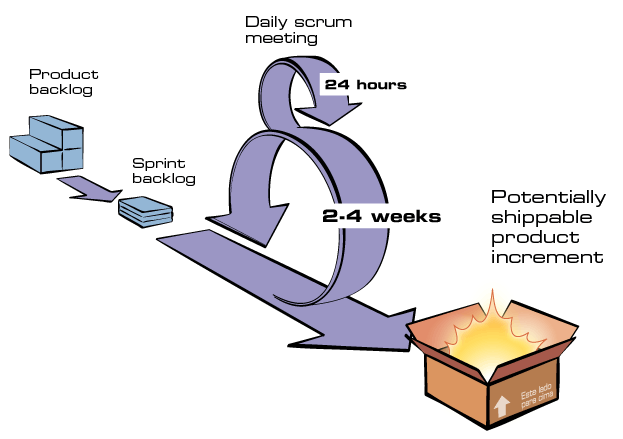
\includegraphics[width=0.75\linewidth]{./figuras/scrum-diagrama}
\caption{Ciclo de vida do \textit{Scrum}}
\label{Fig:cicloScrum}
\legend{Fonte: \cite{desenvolvimento-agil}}
\end{center} 
\end{figure}

Já o \textit{Kanbam} é um quadro onde ficam anotadas as tarefas a serem realizadas. Para o Windbox, ele foi dividido em quatro categorias: tarefas a fazer, tarefas em execução, tare prontas para teste e tarefas concluídas. Conforme as tarefas vão sendo realizadas, os responsáveis vão mudando a posição no quadro. Dessa forma todo o time consegue observar rapidamente o que está sendo feito e o que está pendente.

\section{Modelo de Negócio}
\label{Sec:modeloDeNegocio}

Resolver problemas de engenharia de maneira inovadora é um aspecto crucial no ciclo de vida de um produto, mas encontrar um modelo de negócio que atenda e o torne viável é o diferencial que permite realmente entregar valor para a sociedade.

A expressão "modelo de negócio começou a ser utilizada com frequência, principalmente, após o surgimento dos negócios baseados na internet. O modelo de negócio descreve a lógica de criação, entrega e captura de valor, por parte de uma organização \cite{business-model-generation}. O BMC (\textit{Business Model Canvas}), é um mapa visual que contém nove blocos com os principais elementos de um modelo de negócio. As nove áreas são:

\begin{itemize}
    \item Segmentos de clientes: Define qual é o mercado e o nicho de cliente da oferta de valor.
    \item Oferta de valor: Define qual é o benefício ou valor entregue ao segmento de cliente.
    \item Canais de vendas: Define como a empresa se comunica e entrega valor aos clientes.
    \item Relacionamento com o cliente: Define quais são as estratégias necessárias para fidelizar os clientes.
    \item Fonte de receitas: Define quanto e como os clientes irão pagar pelos benefícios recebidos.
    \item Recursos chaves: Define quais os ativos fundamentais para o modelo de negócio funcione.
    \item Atividades chave: Define quais as atividades mais importantes para a realização do negócio.
    \item Parceiros chave: Define as empresas que ajudaram a entregar a oferta de valor.
    \item Fonte de custos: Define os custos que estão envolvidos na operação do negócio.
\end{itemize}

O BMC da Windbox pode ser visualizado na figura \ref{Fig:bmc-windbox}. Como já foi dito anteriormente, a proposta de valor do Windbox é auxiliar gestores na identificação de problemas na produção dos parques eólicos. O segmento de clientes se restringe inicialmente aos parques eólicos no Brasil. Futuramente, quando o produto estiver consolidado em território nacional, poderá ser comercializado internacionalmente. A principal forma de contato com esses clientes é através de telefonemas e nos principais eventos de energia eólica do país. O licenciamento mensal ou anual da ferramenta é a principal fonte de receita da empresa, que possui como maior fonte de custo a infraestrutura em nuvem que hospeda a solução e recursos humanos. Como a ferramenta está em fase de pre-venda, a maior parte dos custos é mantido por dois parceiros, o BNB e o CNPq, através de fomento, como já foi abordado anteriormente.

\begin{figure}[htbp!] \begin{center}
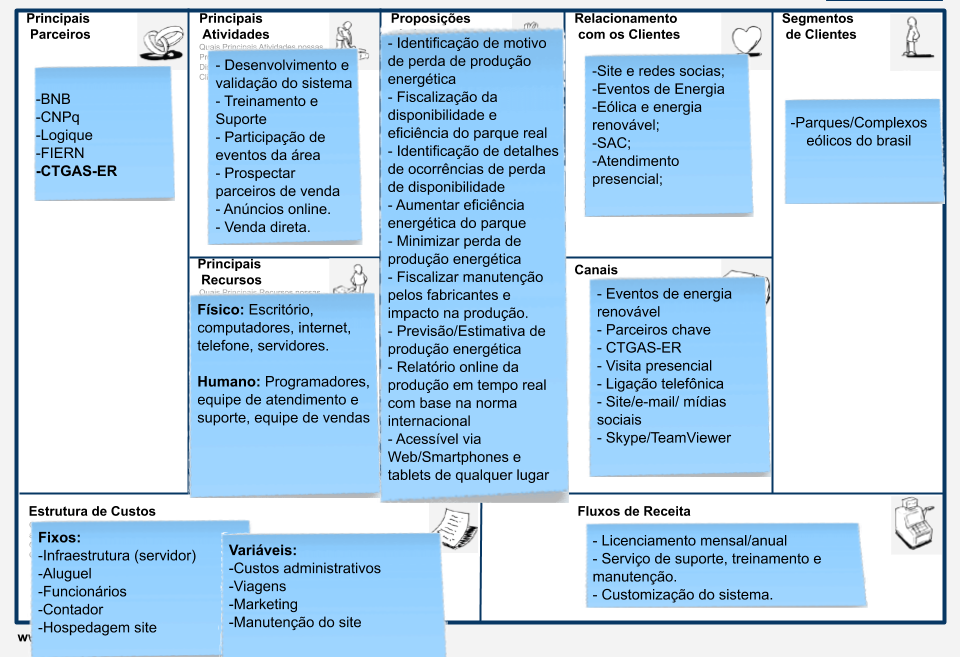
\includegraphics[width=1\linewidth]{./figuras/BMG}
\caption{\textit{Business Model Canvas} do Windbox}
\label{Fig:bmc-windbox}
\end{center} 
\end{figure}

Para compreender mais profundamente a proposta de valor e o segmento de cliente do Windbox, foi utilizado a ferramenta "Canvas de proposta de valor", dos mesmos autores do BMC. O Canvas de proposta de valor funciona como uma especie de detalhamento dos blocos de segmentos de clientes e de proposta de valor do \textit{Business Model Canvas}. A sua principal função é ajudar na compreensão e se aprofundar mais nesses dois blocos chaves do negócio.

O canvas é dividido em dois lados, esquerdo e direito. O lado esquerdo está o mapa de valor, que descreve os aspectos de uma proposta de valor especifica criada por uma empresa. Já do lado direito, está o perfil do cliente, que descreve o segmento de cliente específico.

A figura \ref{Fig:mapa-valor-canvas} demonstra o lado esquerdo (mapa de valor). Ela é dividida em:
\begin{itemize}
    \item Produtos e Serviços: Define todos os produtos e serviços em torno dos quais a proposta de valor é construída.
    \item Analgésicos: Descreve como os produtos ou serviços aliviam a dor do cliente.
    \item Criadores de ganhos: Descreve como os produtos ou serviços geram ganhos para o cliente.
\end{itemize}

\begin{figure}[htbp!] \begin{center}
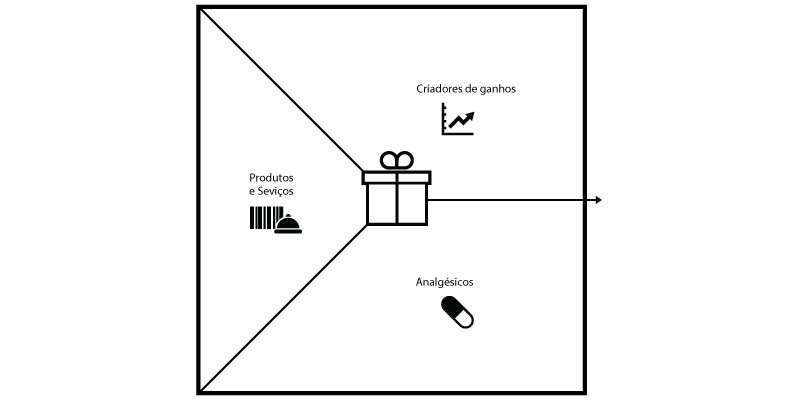
\includegraphics[width=1\linewidth]{./figuras/Mapa-de-Valor-Canvas-de-Proposta-de-Valor}
\caption{Demonstração do mapa de valor}
\label{Fig:mapa-valor-canvas}
\end{center} 
\end{figure}

A figura \ref{Fig:perfil-cliente-canvas} demonstra O lado direito (perfil do cliente). Ela é dividida em: 
\begin{itemize}
    \item Tarefas do cliente: Descreve o que os clientes estão tentando fazer no seu trabalho ou na sua vida.
    \item Dores: Descreve os resultados ruins, os riscos e os obstáculos do cliente.
    \item Ganhos: Descreve os resultados que os clientes querem encontrar.
\end{itemize}

\begin{figure}[htbp!] \begin{center}
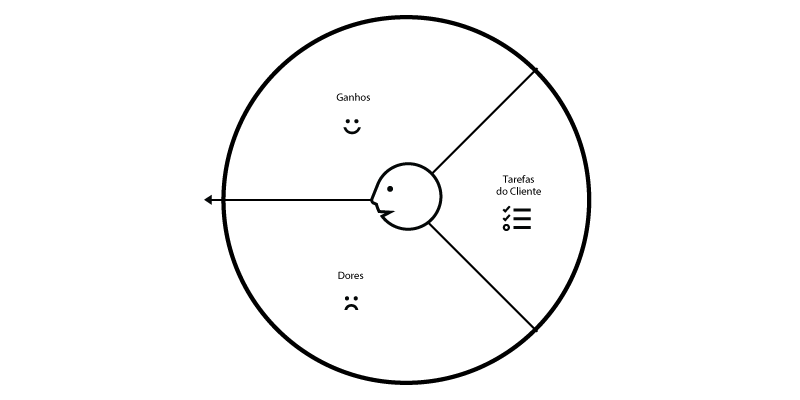
\includegraphics[width=1\linewidth]{./figuras/Perfil-do-Clientes-Canvas-de-Proposta-de-Valor}
\caption{Demonstração do perfil do cliente}
\label{Fig:perfil-cliente-canvas}
\end{center} 
\end{figure}

Na figura \ref{Fig:canvas-valor-windbox} é demonstrado o canvas de valor do Windbox.

\begin{figure}[htbp!] \begin{center}
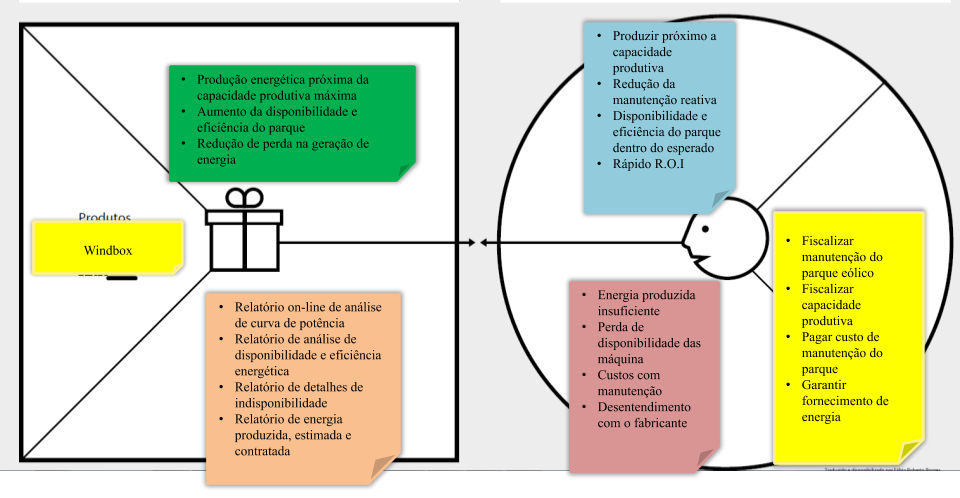
\includegraphics[width=1\linewidth]{./figuras/canvas-de-valor}
\caption{Canvas de valor do Windbox}
\label{Fig:canvas-valor-windbox}
\end{center} 
\end{figure}
